\documentclass[serif,12pt]{beamer}
\usetheme{Antibes}
%\usecolortheme{whale}
\usepackage[utf8]{inputenc}
\usepackage[spanish]{babel}

\usepackage{multicol}

\usepackage{framed}
\usepackage{color}
\usepackage{wrapfig}\definecolor{shadecolor}{RGB}{224,238,238}



\begin{document}

\title[NoSQL in VO to support Big Data]{Integrating NoSQL into VO to support Big Data Challenges}  
\institute[UGR]{TFM - Máster en Métodos y Técnicas Avanzadas en Física}
\author[José Antonio Magro Cortés]{José Antonio Magro Cortés}
\date[Septiembre 2013]


%%%%%%%%%%%%%%%%%%%%%%%%%%%%%%%%%%%%%%%%%%%%%%%%%%%%%%%%%%%%%%%%%%%%%%%%%%%%%%%%%%%%%%%
% dia 1 - título
\begin{frame}
\titlepage
\end{frame}
%%%%%%%%%%%%%%%%%%%%%%%%%%%%%%%%%%%%%%%%%%%%%%%%%%%%%%%%%%%%%%%%%%%%%%%%%%%%%%%%%%%%%%%



%%%%%%%%%%%%%%%%%%%%%%%%%%%%%%%%%%%%%%%%%%%%%%%%%%%%%%%%%%%%%%%%%%%%%%%%%%%%%%%%%%%%%%%
% dia 2 - contenido
\begin{frame}
\frametitle{Contenido}
\tableofcontents
\end{frame} 
%%%%%%%%%%%%%%%%%%%%%%%%%%%%%%%%%%%%%%%%%%%%%%%%%%%%%%%%%%%%%%%%%%%%%%%%%%%%%%%%%%%%%%%



%%%%%%%%%%%%%%%%%%%%%%%%%%%%%%%%%%%%%%%%%%%%%%%%%%%%%%%%%%%%%%%%%%%%%%%%%%%%%%%%%%%%%%%
% dia 3 - objetivo
\section{Objetivo}
\begin{frame}
\frametitle{Objetivo}


Realizar un estudio sobre la problemática de \emph{Big Data} en astronomía y proponer tecnologías alternativas a las existentes, dentro del Observatorio Virtual.


\end{frame}
%%%%%%%%%%%%%%%%%%%%%%%%%%%%%%%%%%%%%%%%%%%%%%%%%%%%%%%%%%%%%%%%%%%%%%%%%%%%%%%%%%%%%%%



%%%%%%%%%%%%%%%%%%%%%%%%%%%%%%%%%%%%%%%%%%%%%%%%%%%%%%%%%%%%%%%%%%%%%%%%%%%%%%%%%%%%%%%
% dia 4 - motivación
\section{Motivación}
\begin{frame}
\frametitle{Motivación}


\begin{itemize}
\item A raíz del curso \emph{Archivos Astronómicos: El Observartorio Virtual} (MTAF):
  \begin{itemize}
  \item Problemas en la gestión de grandes cantidades de datos
  \item Inadecuación de:
    \begin{itemize}
    \item DBMS
    \item Formatos
    \item Tecnologías
    \end{itemize}
  \end{itemize}
\end{itemize}

\end{frame}
%%%%%%%%%%%%%%%%%%%%%%%%%%%%%%%%%%%%%%%%%%%%%%%%%%%%%%%%%%%%%%%%%%%%%%%%%%%%%%%%%%%%%%%


\section{Big Data}
%%%%%%%%%%%%%%%%%%%%%%%%%%%%%%%%%%%%%%%%%%%%%%%%%%%%%%%%%%%%%%%%%%%%%%%%%%%%%%%%%%%%%%%

%%%%%%%%%%%%%%%%%%%%%%%%%%%%%%%%%%%%%%%%%%%%%%%%%%%%%%%%%%%%%%%%%%%%%%%%%%%%%%%%%%%%%%%
% dia 5 - problema
\subsection{Definición}
\begin{frame}
\frametitle{Definición}

\begin{shaded}
\emph{Conjuntos de datos tan grandes y complejos que dificultan su procesamiento mediante los sistemas actuales y tradicionales de gestión de bases de datos. Los problemas principales son la captura, clasificación, sistematización, almacenamiento, búsqueda, compartición, transferencia, análisis y visualización.}
\end{shaded}
\end{frame}
%%%%%%%%%%%%%%%%%%%%%%%%%%%%%%%%%%%%%%%%%%%%%%%%%%%%%%%%%%%%%%%%%%%%%%%%%%%%%%%%%%%%%%%
% dia 6 - problema
\subsection{Problemas}

\begin{frame}
\frametitle{Problemas}

\begin{figure}
\centering
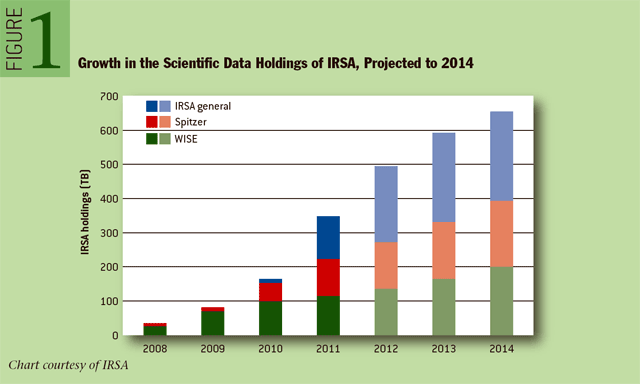
\includegraphics[width=0.7\textwidth, height=0.7\textheight]{images/data_rates.png} 
\label{fig:data_rates}
\end{figure}


\end{frame}
%%%%%%%%%%%%%%%%%%%%%%%%%%%%%%%%%%%%%%%%%%%%%%%%%%%%%%%%%%%%%%%%%%%%%%%%%%%%%%%%%%%%%%%

%%%%%%%%%%%%%%%%%%%%%%%%%%%%%%%%%%%%%%%%%%%%%%%%%%%%%%%%%%%%%%%%%%%%%%%%%%%%%%%%%%%%%%%
% dia 7 - VO
\section{Observatorio Virtual}
\begin{frame}
\frametitle{Observatorio Virtual}

\begin{itemize}
\item FITS
\item TAP
\item OpenCADC
\end{itemize}

\end{frame}
%%%%%%%%%%%%%%%%%%%%%%%%%%%%%%%%%%%%%%%%%%%%%%%%%%%%%%%%%%%%%%%%%%%%%%%%%%%%%%%%%%%%%%%


\section{NoSQL}
%%%%%%%%%%%%%%%%%%%%%%%%%%%%%%%%%%%%%%%%%%%%%%%%%%%%%%%%%%%%%%%%%%%%%%%%%%%%%%%%%%%%%%%
\subsection{Definición}
\begin{frame}
\frametitle{NoSQL}

\begin{center}
NoSQL = \emph{Not Only SQL} \newline
\end{center}


\begin{multicols}{2}

\textbf{Ventajas}
\begin{itemize}
\item Escalabilidad
\item Modelos de datos flexibles
\item Bajo coste
\end{itemize}

\textbf{Inconvenientes}
\begin{itemize}
\item Relativamente reciente
\item Soporte
\item Pocos usuarios
\end{itemize}

\end{multicols}

\end{frame}
%%%%%%%%%%%%%%%%%%%%%%%%%%%%%%%%%%%%%%%%%%%%%%%%%%%%%%%%%%%%%%%%%%%%%%%%%%%%%%%%%%%%%%%



%%%%%%%%%%%%%%%%%%%%%%%%%%%%%%%%%%%%%%%%%%%%%%%%%%%%%%%%%%%%%%%%%%%%%%%%%%%%%%%%%%%%%%%
\subsection{Casos de éxito}
\begin{frame}
\frametitle{NoSQL: Casos de éxito}

\begin{itemize}
\item CMS en el LHC
\item ATLAS Workload Management System
\item Medida de niveles de radiación en Seattle
\end{itemize}


\end{frame}
%%%%%%%%%%%%%%%%%%%%%%%%%%%%%%%%%%%%%%%%%%%%%%%%%%%%%%%%%%%%%%%%%%%%%%%%%%%%%%%%%%%%%%%

\subsection{¿Qué es un documento?}
\begin{frame}
\frametitle{NoSQL: Documentos}

\begin{figure}
\centering
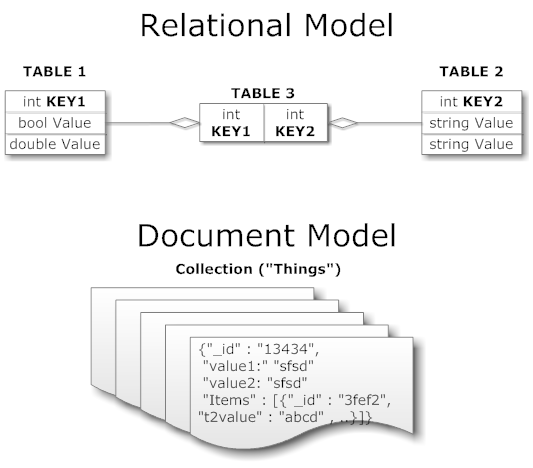
\includegraphics[width=0.8\textwidth, height=0.8\textheight]{images/document_vs_tables.png} 
\label{fig:data_rates}
\end{figure}

\end{frame}

%%%%%%%%%%%%%%%%%%%%%%%%%%%%%%%%%%%%%%%%%%%%%%%%%%%%%%%%%%%%%%%%%%%%%%%%%%%%%%%%%%%%%%%
\subsection{MongoDB}
\begin{frame}
\frametitle{NoSQL: MongoDB}

\begin{itemize}
\item Orientada a documentos
\item Código abierto
\item Soporte completo para índices
\item Fácil instalación y puesta en marcha
\item Balanceo de carga
\item Soporta MapReduce
\item Conexión con Hadoop
\item Tecnología del S. XXI para problemas del S. XXI
\end{itemize}


\end{frame}
%%%%%%%%%%%%%%%%%%%%%%%%%%%%%%%%%%%%%%%%%%%%%%%%%%%%%%%%%%%%%%%%%%%%%%%%%%%%%%%%%%%%%%%

%%%%%%%%%%%%%%%%%%%%%%%%%%%%%%%%%%%%%%%%%%%%%%%%%%%%%%%%%%%%%%%%%%%%%%%%%%%%%%%%%%%%%%%
\section{NoSQL en el VO}
\begin{frame}
\frametitle{NoSQL en el VO}

\begin{itemize}
\item Almacén FITS
\item MapReduce para registros
\item Conexión OpenCADC y NoSQL para ALMA
\end{itemize}


\end{frame}
%%%%%%%%%%%%%%%%%%%%%%%%%%%%%%%%%%%%%%%%%%%%%%%%%%%%%%%%%%%%%%%%%%%%%%%%%%%%%%%%%%%%%%%


%%%%%%%%%%%%%%%%%%%%%%%%%%%%%%%%%%%%%%%%%%%%%%%%%%%%%%%%%%%%%%%%%%%%%%%%%%%%%%%%%%%%%%%
\section{Conclusiones y trabajo futuro}
\begin{frame}
\frametitle{Conclusiones y trabajo futuro}

\begin{multicols}{2}

\textbf{Conclusiones}
\begin{itemize}
\item NoSQL más eficiente para algunos problemas
\item Menor coste para análisis y diseño
\item Facilidad para incorporar frameworks de VO a NoSQL
\end{itemize}

\textbf{Trabajo futuro}
\begin{itemize}
\item Adaptar OpenCADC a NoSQL
\item Usar métricas formales de diseño
\item Benchmarks para medir rendimiento
\end{itemize}

\end{multicols}

\end{frame}
%%%%%%%%%%%%%%%%%%%%%%%%%%%%%%%%%%%%%%%%%%%%%%%%%%%%%%%%%%%%%%%%%%%%%%%%%%%%%%%%%%%%%%%

\end{document}
